\section{Preliminary Results}
\label{sec:results}
One of the most important initial goals of \flux\ is to gain
a fundamental understanding of key design challenges pertaining
to the new RM paradigm shift.
In the context of \flux's run-time system, the scalability
and productivity
challenges---as described in Section~\ref{sect:challenges}---are especially
relevant and crucial. 
%Clearly, we  must provide a wide range
%of run-time elements such as parallel programming models,
%tools and middleware with performance, scalability, easy integration
%and interoperability.
Thus, this section evaluates our prototype's performance
and scalability characteristics as well as its ability
to support various productivity software programs. 

One of the most important initial goals of \flux\ is to gain
a fundamental understanding of key design challenges pertaining
to the major shift in the new RM conceptual model.
In the context of \flux's run-time system, the scalability
and productivity
challenges---as described in Section~\ref{sect:challenges}---are especially
relevant and crucial. Clearly, we  must provide a wide range
of run-time elements such as parallel programming models,
tools and middleware with performance, scalability, easy integration
and interoperability.
This section evaluates our prototype's performance
and scalability characteristics as well as its ability
to support various HPC run-time elements.


\subsection{KVS Access Patterns (KAP) Tester}
To examine the performance of \flux's run-time system,
we developed a tester called KVS Access Patterns (KAP).
\begin{figure}
  \centering
  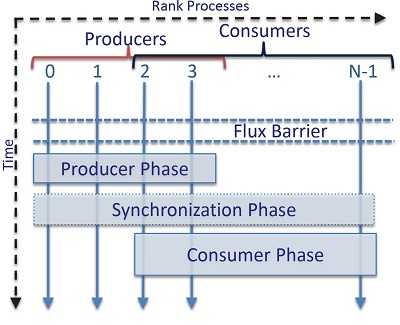
\includegraphics[scale=0.45]{kaptester}
  \caption{Main phases of KAP tester}
  \label{fig:kap}
\end{figure}
KAP models KVS access patterns through various interactions
between KVS writers and readers. Writers are called producers;
readers consumers.
In essence, KAP allows a configurable number of producer processes
to write key-value objects into our KVS 
and a configurable number of consumers to read these
objects after ensuring the consistent KVS state.

In addition to producer and/or consumer counts,
KAP provides a range of parameters that can affect performance.
Among them include the value size (of key-value objects),
the number of objects to put,
the number of objects to read, objects access 
patterns (through different striding), and
synchronization primitives used for consistency.

Figure~\ref{fig:kap} shows the three main phases of KAP.
Right after tester processes are launched into a set of nodes
in which a CMB session had been established,
they are assigned to ranks such that consecutive rank
processes are distributed to consecutive nodes.
Then, the rank processes determine their roles based
on the command line arguments and issue a named barrier
that \flux\ provides to begin to play their roles
simultaneously.

Next, each producer calls the specified number of
{\tt kvs\_put}s of an object of the specified value size.
For each call, the producers use unique keys, but
the values can be configured to be either unique
or redundant.
Once this producer phase completes, all of the producers and consumers
participate in a consistency protocol that uses
\flux's synchronization primitives such as the collective
fence---i.e., the {\tt kvs\_fence} function.
Finally, during the consumer phase, consumers read
these key-value objects by calling {\tt kvs\_get}s.
KAP provides options to emulate various read access
patterns.


\subsection{Experimental Setup}
We run all of our experiments on two Linux clusters installed at LLNL,
named Zin and Cab.
Each compute node of these clusters has 2 sockets and 32 GB of RAM.
Each socket is populated with an 8-core 2.6 GHz Intel
Xeon E5-2670 processor, resulting in 16 cores per node.
Zin consists of 2,916 compute nodes totaling 46,656 cores;
Cab is a smaller system with the same node type,
consisting of 1,296 compute nodes with a total of 20,736 cores.
Nodes are connected by a Qlogic Infiniband QDR interconnect.
The largest allocation allowed in normal batch mode
is 258 nodes on Cab and 512 on Zin.

We run KAP with varying arguments to its parameters
in batch mode and collect various 
performance metrics. 
Because the exploration
space is huge, however, we limit our experiments with
only a subset of the parameter set and of sampling points.

Specifically, we run our KAP tests at 64, 128, 256 and 512
compute nodes, and always fully populate each node with
16 processes, each acting as consumer or producer or
both. We vary the consumer or producer count
while fixing the other at the total number of cores.
We also vary the value size 
from 8 Bytes to 32 Kilobytes in the powers of 8,
and the key-value object access count of each consumer
from 1 to the total process count.

Further, we evaluate the performance impact 
of how key-value objects are organized 
in KVS by either storing all of the objects into a single KVS directory
or distributing them into multiple directories---i.e.,
128 objects per KVS directory.
Finally, we study the performance implications of 
redundancy in values by either configuring producers to generate
unique or redundant values across them.

For simplicity, we configure the topology of CMB only as 
the binary tree and and use \flux's collective fence 
as our only mechanism to enforce consistency.

\subsection{Performance Results and Analysis}
\label{results}
Of tens of thousands of our sampling runs, we find that the fully populated
cases---i.e. both producer and consumer counts become equal to the total
process count---are most revealing. In particular, we carefully analyze 
the maximum latency of each of the main phases of KAP for these cases 
because this metric represents the critical path of the performance of
many HPC services. For example, distributed 
HPC software would use KVS operations in a coordinated fashion to exchange 
connection information among processes during its bootstrapping 
phase~\cite{LIBI,PMI2}. Unless {\em all} 
of the distributed processes complete their
KVS operations, their communication fabric cannot be established. 

\begin{wrapfigure}{l}{80mm} 
  \centering
  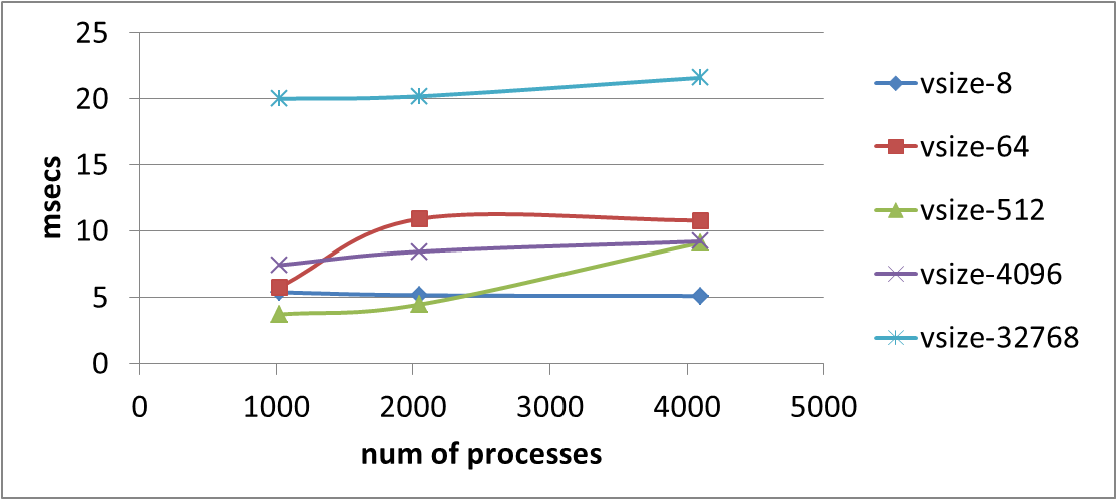
\includegraphics[scale=0.40]{producer}
  \caption{Max latency of producer phase}
  \vspace{-.5cm}	
  \label{fig:prod}
\end{wrapfigure}

Figure~\ref{fig:prod} shows the maximum latency of the producer phase
for these cases. Essentially, these lines indicate how well {\tt kvs\_put}
scales as we increase the number of producers. Each line represents
different value sizes---e.g., vsize-8 refers to value size being
8 Bytes. As shown in this graph, the {\tt kvs\_put} simply performs and
scales well. This matches our expectations because the key-value objects
are locally cached at {\tt kvs\_put} time and pushed to the
server at the next consistency event. 

\ifcomments
\marginpar{\tiny DA: I will add data from 8K if I get it on Zin in time.}

\begin{figure}[ht]
\centering
\begin{subfigure}[With unique values]{
  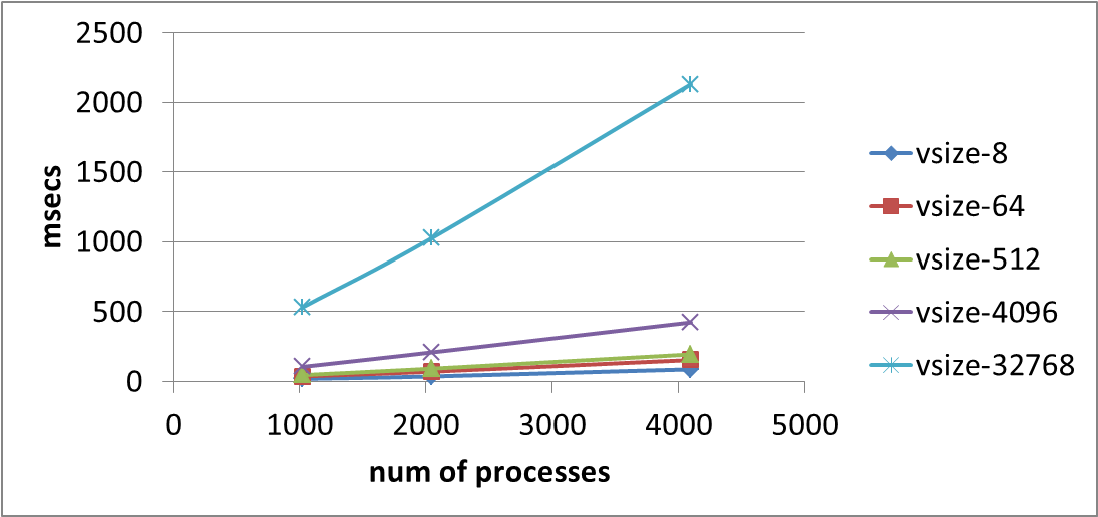
\includegraphics[width=.75\linewidth]{sync}
  \label{fig:sync:noredund}
}%
\end{subfigure}
\begin{subfigure}[With redundant values]{
  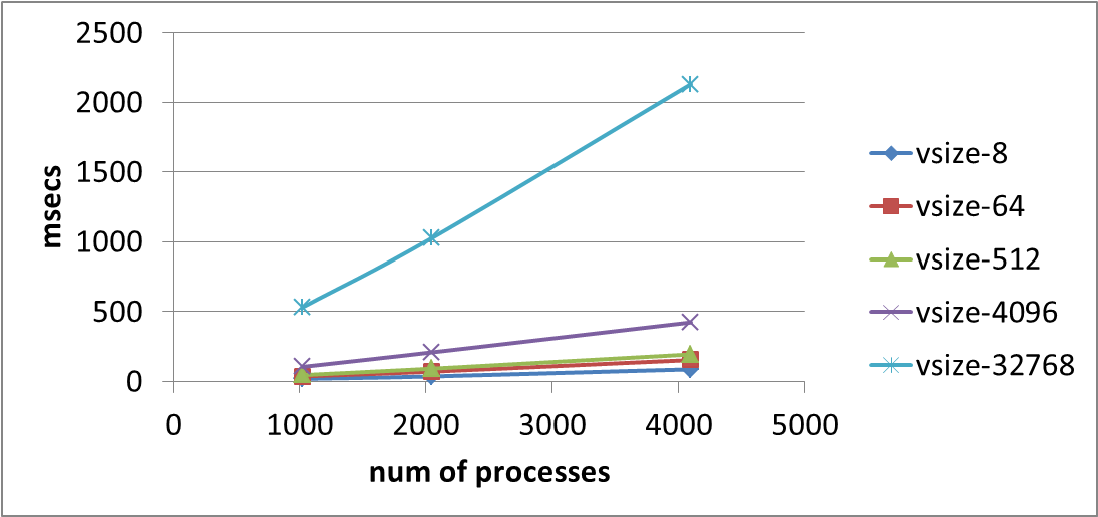
\includegraphics[width=.75\linewidth]{sync}
  \label{fig:sync:redund}
}%
\end{subfigure}
\caption{Max latency of synchronization phase}
\label{fig:sync}
\end{figure}


Moving onto the synchronization phase, Fig.~\ref{fig:sync} shows 
how well {\tt kvs\_fence} scales during this phase,
as we increase the number of producers. 
As with the producer latency,
each line represents different value sizes.  
The most revealing observation is that 
fence scalabilty appears to depend on the level of
redundancy in key-value objects that had previously 
been put in. Figure~\ref{fig:sync:redund} 
shows the maximum latency of the synchronization phase
when redundant values are used. It scales
far better than Fig.~\ref{fig:sync:noredund}
where there is zero redundancy in values. 
We theorize that in the former case, fence performs linearly with respect to the number of
producers because these unique values are being {\em concatenated} while
being sent up the tree. It performs logarithmically for the latter case
because redundant values are being {\em reduced} while being sent 
up the tree. %%(MENSION R^2 here?)

\marginpar{\tiny DA: I am speculating a bit for redundant case; my job on cab will confirm or deny this.}

\begin{figure}[ht]
\centering
\begin{subfigure}[With single-directory layout]{
  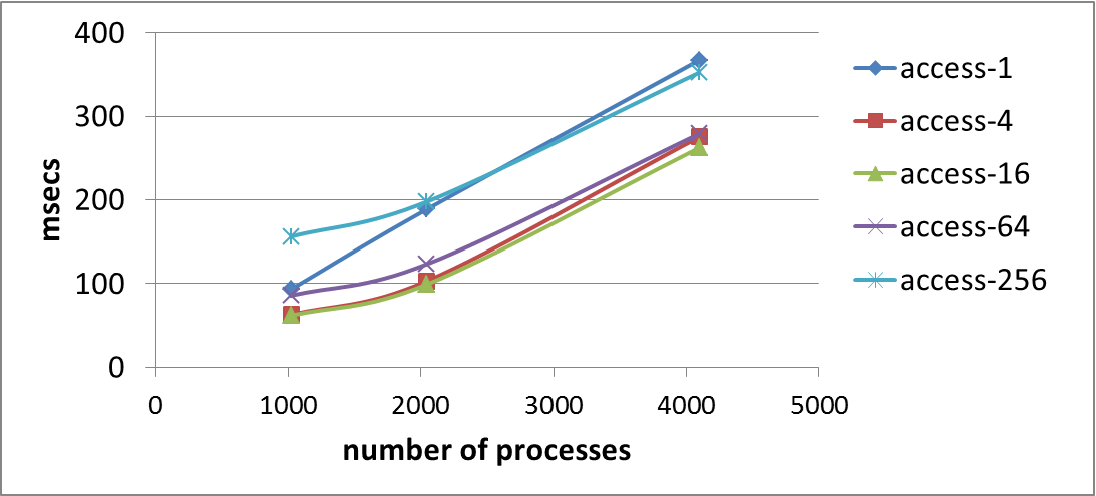
\includegraphics[width=.75\linewidth]{consumer-1-dir}
  \label{fig:cons:dir}
}%
\end{subfigure}
\begin{subfigure}[Improvements with multiple directories]{
  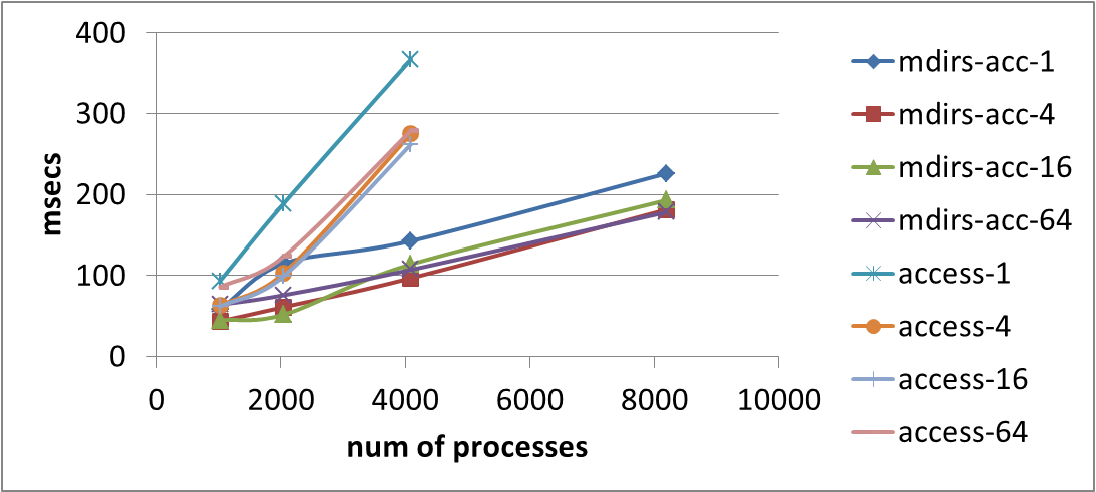
\includegraphics[width=.75\linewidth]{consumer-dist-dir}
  \label{fig:cons:dirs}
}%
\end{subfigure}
\caption{Max latency of consumer phase (value size: 8 Bytes)}
\vspace{-.5cm}
\label{fig:consumer}
\end{figure}

Figure~\ref{fig:consumer} shows the maximum latency of the consumer
phase with respect to various parameter settings. 
The lines generally suggest how well {\tt kvs\_get}
scales, as we increase the number of consumers. Each line represents
the latency when each consumer reads different numbers of 
key-value objects---e.g., access-4 refers to read 4 distinct key-value 
objects. While these figures show only the performance of reading
objects with 8-Byte value, we observe that the general 
scalability trends are similar at different value sizes.

Figure~\ref{fig:cons:dir} shows the maximum latency of {\tt kvs\_get}
when the target key-value objects are all stored in a single
KVS directory. The latency is quite high and also increases
linearly, as we increase the number of consumers. 
It appears that the poor performance and scaling behavior 
are attributed to KVS replication granularity and 
the fact that the objects are stored in a single directory.

When {\tt kvs\_get} cannot be satisfied by the local KVS replica,
our system ensures that the entire directory where
the requested object resides is replicated on
all of the ancestor CMB daemons that are along the direct path 
to the root. With our access pattern where all objects
are read collectively by consumers, this means the latency is 
$log_2(C) \times T_{replicate}(G)$, where C is the consumer count, and G is the 
total amount of data in the master KVS server.
Thus, the max latency increase for every doubling of consumers is 
$\frac{log_2(2C) \times T_{replicate}(2G)}{log_2(C) \times T_{replicate}(G)}$.
Generally, this would approach 2, 
as we continue to increase the number of consumers,
and our data match with this model.

We can improve this behavior by storing objects across multiple
directories. With such an organization, the size of replicas 
would decrease as we go down the CMB tree. This is of course only when
each consumer reads only a small fraction of data. In another
word, if each consumer read all of the data in KVS, the latency
would be same as the single directory case. 
Figure~\ref{fig:cons:dir} shows the improvements 
when we spread objects into multiple directories by
keeping the number of objects per directory constant: 128.
Label {\tt mdir-acc-k} refers to the same access pattern as {\tt access-k} 
except the accessing objects are stored across multiple directories.


For the case where the size of replicas 
decreases as a function of tree levels, 
we can model the latency as a geometric series. For example, at tree height being $h$,
the latency would be 
$T_{replicate}(G) + T_{replicate}(\frac{G}{2}) + T_{replicate}(\frac{G}{4}) + ... + T_{replicate}(\frac{G}{2^h})$, 
where each term represents the latency of replication per level.
This would approach $2T_{replicate}(G)$. Thus, its improvement over the single
directory scheme is: $\frac{log_2(C) \times T_{replicate}(G)}{2 T_{replicate}(G)}$.
Roughly speaking, the improvements would be on the order of 
$\frac{1}{2}log_2(C)$. The improvements would be linearly 
greater as we increase the scale and our measurements agree with this. 

While significant, we note that a smarter KVS data layout scheme alone
can still fall short of reaching extreme scale. Our model tells us that the latency
will grow linearly when $G$ grows with the scale. 
Say, $G$ doubles every time you double the number of consumers, our geometric series
model predicts the latency will also double:
$\frac{2T_{replicate}(2G)}{2T_{replicate(G)}}$ becomes 
on the order of 2. With the current scheme, the only true way to gain logarithmic
scaling is when $G$ stays constant regardless of scale. 
In a later section, we will discuss some of our plans 
to exploit the understanding we gain from the evaluation. 



